\documentclass[xetex]{beamer}

\usepackage{fontspec}
%\usepackage{xeCJK}
%\setCJKmainfont{Noto Sans CJK SC}
%\newfontfamily\Libertine[Mapping=tex-text]{Linux Libertine O}
\usetheme{Madrid}
\usecolortheme{crane}
\usepackage{graphicx}

\usepackage{polyglossia}
\setdefaultlanguage{english}
\newfontfamily\englishfont[Ligatures=NoCommon]{Linux Libertine O}
% \setotherlanguage{arabic}
% \newfontfamily\arabicfontsf[Script=Arabic]{Noto Naskh Arabic}
\setotherlanguage{chinese}
\newfontfamily\chinesefontsf[Script=CJK]{Noto Sans CJK SC}
\setotherlanguage{yue}
\newfontfamily\yuefontsf[Script=CJK]{Noto Sans CJK TC}

\setotherlanguage{japanese}
\newfontfamily\japanesefontsf[Script=CJK]{Noto Sans CJK JP} % Japanese font
\setotherlanguage{korean}
\newfontfamily\koreanfontsf[Script=CJK]{Noto Sans CJK KR} 
\setotherlanguage{thai}
\newfontfamily\thaifontsf[Script=Thai]{Noto Sans Thai}

\newfontfamily{\silipa}{Noto Serif}
\newcommand{\IPA}[1]{{\silipa\selectfont #1}}

\usepackage{natbib}

\usepackage{mygb4e}
\newcommand{\yueb}[1]{\yuefontsf\selectfont #1}
\renewcommand{\eachwordone}{\yueb}
\renewcommand{\eachwordtwo}{\yueb}
\usepackage[e,f]{mtg2e}
\usepackage{xcolor}
\renewcommand{\mtcitestyle}[1]{\textcolor{teal}{\textit{#1}}}
\newcommand{\msa}{\mtciteform}
\newcommand{\zsm}{\mtciteform}
\newcommand{\ko}{\mtciteform}
\newcommand{\zh}{\mtciteform}
\newcommand{\jpn}{\mtciteform}
\newcommand{\ar}{\mtciteform}
\newcommand{\txx}[1]{\textcolor{blue}{\textbf{#1}}}

\title{Communication and Culture}
\author{Francis Bond}
 
\date{}

\begin{document}

\frame{\titlepage}

% Introduction Slide
\begin{frame}
\frametitle{Introduction to Communicative Competence}
\begin{itemize}
    \item Speaking well goes beyond grammar: it includes situational language choices.
    \item Distinction between linguistic competence and communicative competence.
    \item Focus on East and Southeast Asian languages.
    \item Topics covered: proverbs, speech styles, honorific systems, communicative style.
\end{itemize}
\end{frame}

% Word Skills Slide Series
\section{Word Skills in East and Southeast Asian Languages}
\begin{frame}
\frametitle{Proverbs and Sayings}
\begin{itemize}
    \item Proverbs are central to communication, especially in Malay (peribahasa).
    \item Express social norms and values with cultural references.
    \item Examples encapsulate lessons or advice.
    \item Often used to depersonalize comments, presenting them as traditional wisdom.
    \item Culturally rich and expressive forms such as pantun quatrains.
\end{itemize}
\end{frame}

\begin{frame}
\frametitle{Examples of Malay Proverbs}
\begin{exe}
    \ex \gll Ada hujan, ada panas, ada hari boleh balas. \\
        There rain, there {hot weather}, there day can repay.\\
        \trans `Every action, good or bad, will be repaid in kind.'
    \ex \gll {Sedikit-sedikit lama-lama} jadi bukit. \\
        {Little by little}, become mountain.\\
        \trans `Small, patient actions bring big results.'
\end{exe}
\end{frame}

% Elaborate Expressions Slide Series
\begin{frame}
\frametitle{Elaborate Expressions}
\begin{itemize}
    \item Common in Southeast Asia, with four-syllable compounds (ABAC, ABCB).
    \item Thai, Lao, Vietnamese, and Chinese use these expressions for fluency.
    \item Used to convey deeper cultural meanings and imagery.
    \item Chinese examples (chéng yǔ) reflect historical, literary roots.
\end{itemize}
\end{frame}

\begin{frame}
\frametitle{Examples of Thai Elaborate Expressions}
\begin{table}[]
\centering
\begin{tabular}{lll}
    \textbf{Expression} & \textbf{Literal} & \textbf{Meaning} \\
    \hline
    hǔu-pàa-taa-thı̀ & ear-forest-eye-forest & to be ignorant \\
    phûut-yàang-tham-yàang & speak-kind-do-kind & say one thing, do another \\
\end{tabular}
\end{table}
\end{frame}

\begin{frame}{What are Chengyu (\textchinese{成语})?}
  \begin{itemize}
  \item Chengyu are prototypically four-character, non-compositional
    phrases derived from historical lore or classical literature.
  \item Some are partly compositional
  \item Many are completely non-compositional
  \item They function as lexemes in sentences
  \item They are  more vivid than normal lexemes
  \item There is no definitive list ---- different lexicons range
    from samples of a few hundred up to 50,000 or more
  \item Many excellent (paper) dictionaries exist
  \end{itemize}
\end{frame}     


     \begin{frame}{Some Examples of Chengyu}
       \hfill 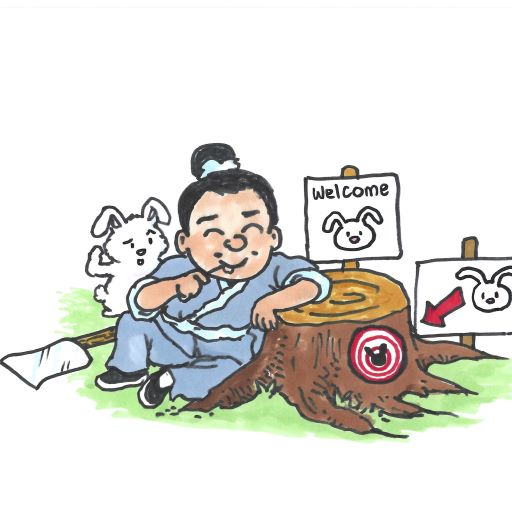
\includegraphics{pics/shouzhudaitu.jpg}
       \vspace{-3cm}
       \begin{exe}
         \ex\label{s:rabbit}
         \glll 守 株 待 兔 \\
         shou zhu dai tu \\
         guard {tree root} wait rabbit \\
         \trans Lit: to wait by a tree for a rabbit
         \trans to expect fortune without putting in any effort
         \ex\label{s:divide}
         \glll 分 崩 离 析 \\
         fen beng li xi \\
         divide rupture leave {split apart} \\
         \trans to completely fall apart
       \end{exe}

Image from \href{https://www.dimsumwarriors.com/chengyu/守株待兔-shouzhudaitu/}{Yumcha Studios}
     \end{frame}
     \begin{frame}{Many come from stories}

     
  During the Spring and Autumn period, there was a farmer (\textchinese{农民} Nóngmín) who had a tree in his field. He would frequently rest under a tree after a long day of working.

One day, he was working in the field and saw a scared rabbit come running past him, crash into that tree, and die suddenly. The farmer was overjoyed! He had just gotten a free dinner without having to put in any work.

While eating rabbit stew that night, the farmer had a thought. “Why even bother farming, when I have a tree that rabbits just ran into?” The farmer really liked this thought and from that day forth, he abandoned his plow to simply sit by the tree and wait for another rabbit to run into it and die.

However, to the farmer’s surprise, no more rabbits crashed into the tree again ever again. Overtime, the farmer ended up with barren fields, impoverished, and the laughing stock of the village.


\url{https://www.tutormandarin.net/en/holding-a-tree-and-waiting-for-a-rabbit/}
\end{frame}

\begin{frame}{Distribution of Chengyu in different Genres}
    \begin{center}
      \begin{tabular}{lrrrr}
        \textbf{Genre} & \textbf{Sents} &
        \multicolumn{3}{c}{\textbf{Chengyu}} \\
        &  &
        \textbf{Types} &  
        \textbf{Tokens} &  \textbf{Tokens/100 Sents} \\
        \hline
        Story   &  1,226  &   138  &    153  & 7.3 \\
        News    &  2,138  &   225  &    312  & 7.5 \\
        Essay   &    816  &   180  &    227  & 15.6 \\
        Tourism &  3,280  &   538  &    962  & 11.8 \\
        \hline
        Total   &  7,460  &  1,003  &  1,654  & 10.3 \\
      \end{tabular}
    \end{center}
    \begin{itemize}
    \item The essay \textit{Cathedral and the Bazaar} has the most,
      which fits well with its intellectual tone.
    \end{itemize}

    From \citet{Ho:Kng:Wang:Bond:2014}.

    Used more in Chinese, then Korean, then Japanese.
  \end{frame}
  
  
\begin{frame}{Comparison with the West}
  \begin{itemize}
  \item These are not so different from Western proverbs (IMHO)
    \begin{itemize}
    \item Many of which come from classic works
      \\ Aesop's fables, the Bible, Homer, ...
    \item Using them correctly is a sign of erudition
    \end{itemize}
  \item Chéngyǔ often require a degree of interpretation, as their
    literal meaning may differ from the figurative message they
    convey. For example, the chéngyǔ \textchinese{画蛇添足} \zh{huà shé tiān zú},
    ``to draw legs on a snake'', means ``to add something
    superfluous'', warning against unnecessary embellishments.  But this is also true for the English expression ``like lipstick on a pig'' or an expression like ``sour grapes'', \ldots
  \item Because of their semi-fixed form (normally 4, sometimes 5 characters) they are more distinct from normal text.
  \end{itemize}
\end{frame}


\begin{frame}{Auspicious and Inauspicious Words in Cantonese}

\begin{tabular}{lll}
%\hline
% \textbf{Word} & \textbf{Pronunciation} & \textbf{Meaning / Association} \\
% \hline
\multicolumn{3}{l}{\textbf{Auspicious Words}} \\
\hline
\textyue{八} (eight) & \textyue{baat} & $\approx$ \textyue{發} (faat) ``prosperity'' \\
\textyue{橙} (tangerine) & \textyue{daaih gāt} & $\approx$ \textyue{大吉} (daaih gāt), ``great fortune" \\
\textyue{魚} (fish) & \textyue{yú} & $\approx$ \textyue{餘} (yùh), ``abundance" \\
\textyue{金} (gold) & \textyue{gām} & Symbolizes wealth and prosperity \\
\textyue{生菜} (lettuce) & \textyue{sāang chòih} & $\approx$ \textyue{生財} (sāang chòih), ``making money" \\[1ex]

\multicolumn{3}{l}{\textbf{Inauspicious Words}} \\
\hline
\textyue{四} (four) & \textyue{sei} & $\approx$ \textyue{死} (séi), ``death" \\
\textyue{書} (book) & \textyue{syū} &$\approx$ \textyue{輸} (syū), ``to lose" \\
\textyue{空} (empty) & \textyue{hūng} & Associated with emptiness or misfortune \\
\textyue{鞋} (shoe) & \textyue{hái} & $\approx$ \textyue{孩} (hái), associated with failure \\
\textyue{舌} (tongue) & \textyue{siht} & $\approx$ \textyue{失} (siht), ``to lose" \\
\hline
\end{tabular}

\medskip

So we give and receive tangerines on New Year's Day!

\end{frame}

% Slide 1
\begin{frame}
\frametitle{Introduction to Speech Styles}
\begin{itemize}
    \item Many East and Southeast Asian languages use different speech styles (registers).
    \item Speech styles convey respect, social distance, and familiarity.
    \item Marked by pronunciation, vocabulary, particles, morphology, and syntax.
    \item Styles are often culturally codified, such as in Javanese and Korean.
    \item Speakers are mindful of using appropriate styles in various social situations.
\end{itemize}
\end{frame}

% Slide 2
\begin{frame}
\frametitle{Speech Styles in Thai}
\begin{itemize}
    \item Thai has styles like public, consultative, and personal (informal).
    \item Consultative style uses particles \textit{khráp} (male) and \textit{khâ} (female).
    \item Particles show respect and are used at sentence ends or alone.
    \item Requires careful pronunciation and elevated vocabulary.
    \item Politeness demands avoiding abrupt or negative expressions.
\end{itemize}
\end{frame}

% Slide 3
\begin{frame}
\frametitle{Thai Greeting Styles}
\begin{itemize}
    \item Physical greetings also reflect social hierarchy.
    \item The traditional Thai \textit{wai} has variations based on social rank.
    \item Higher-ranked individuals may have more relaxed gestures.
    \item Verbal and non-verbal etiquette combine to convey respect.
\end{itemize}
\begin{center}
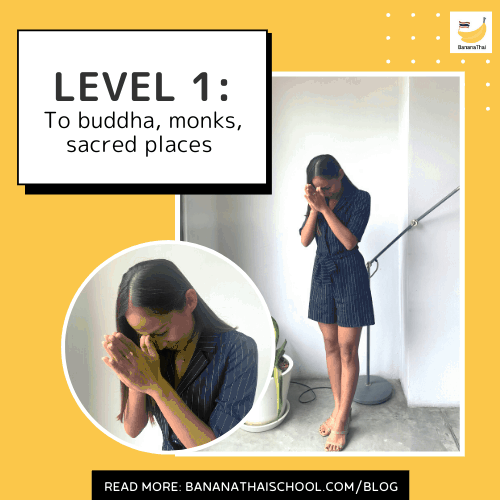
\includegraphics[width=0.23\textwidth]{pics/wai-1.png}

\includegraphics[width=0.23\textwidth]{pics/wai-2.png}
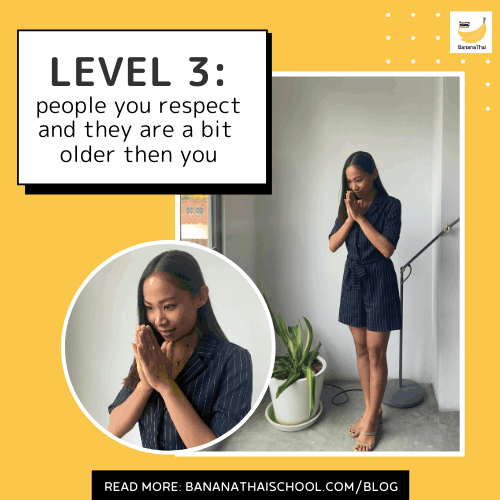
\includegraphics[width=0.23\textwidth]{pics/wai-3.png}

\includegraphics[width=0.23\textwidth]{pics/wai-4.png}
\end{center}
\end{frame}

% Slide 4
\begin{frame}
\frametitle{Speech Styles in Javanese}
\begin{itemize}
    \item Javanese features highly developed vocabulary levels.
    \item Primary styles: \textit{ngoko} (informal) and \textit{krama} (formal, respectful).
      \begin{itemize}
      \item  \textit{Ngoko} is personal and direct, typically for close relations.
      \item[] used for thinking to oneself
         \item  \textit{Madya} is a compromise between conflicting criteria of
           age, social standing, and familiarity.
           \item[] it uses abbreviated krama words with ngoko affixes
    \item \textit{Krama} includes set phrases, indirect expressions, and formal tone.
    \item[] used to address superiors or strangers, aiming for social smoothness.

      
      \end{itemize}
\end{itemize}
\end{frame}

% Slide 5
\begin{frame}
\frametitle{Javanese Speech Style Examples}
\begin{table}[]
\centering
\begin{tabular}{lll}

\textbf{Ngoko} & \textbf{Krama} & \textbf{Meaning} \\
\hline
omah & griya & house \\
wong & tiyang & person \\
lunga & késah & go \\
sapi & lembu & cow \\
mati & pejah & die \\

\end{tabular}
\end{table}

‘What’ is \msa{apa} in ngoko, \msa{napa} in madya, punapa in \msa{krama}.

\end{frame}


% Slide 7
\begin{frame}
\frametitle{Speech Styles in Sasak (Lombok)}
\begin{itemize}
    \item Sasak has three main speech levels: low, mid, and high.
    \item High-level vocabulary reserved for addressing higher-status individuals.
    \item Style level choice depends on the addressee's social rank.
    \item Limited to around 180 words compared to Javanese's extensive system.
    \item Example phrase for “Have you eaten?” changes across levels.
      \begin{tabular}{ll}
      \textbf{Low} & Wah-m mangan kamu? \\
      \textbf{Mid} & Wah-m medaran side? \\
      \textbf{High}&  Sampun-m majengan pelinggih?  \\
    \end{tabular}
  \end{itemize}
\end{frame}

% Slide 9
\begin{frame}
\frametitle{Speech Styles in Korean}
\begin{itemize}
    \item Korean speech styles, known as \textit{che}, differ by verb endings.
    \item Five primary styles: plain, banmal, familiar, polite, and formal.
    \item Style choice depends on age, social rank, and relationship.
    \item Example: \ko{haeyo-che} (polite) for general politeness.
    \item \ko{Hapsyo-che} (formal) for respectful or professional contexts.
\end{itemize}
\end{frame}

% Slide 10
\begin{frame}
\frametitle{Korean Speech Style Examples}
\begin{table}[]
\centering
\begin{tabular}{lll}
\textbf{Speech Style} & \textbf{Example} & \textbf{Meaning} \\ \hline
Plain    & \ko{bi ga o-nda} & It is raining \\
Banmal   & \ko{bi ga o-a} & It is raining \\
Familiar & \ko{bi ga o-ne} & It is raining \\
Polite   & \ko{bi ga o-ayo} & It is raining \\
Formal   & \ko{bi ga o-bnita} & It is raining \\
\end{tabular}
\end{table}
\end{frame}

% Slide 11
\begin{frame}
\frametitle{Changing Speech Styles in Korean}
\begin{itemize}
    \item Moving to banmal signals closeness and familiarity.
    \item Expressed as "putting down the language."
    \item Verb endings change based on relationship status.
    \item Politeness levels can shift with changes in relationships.
    \item People are very aware of the levels
      \begin{exe}
        \ex \ko{Uri neun seoro hage-haneun sai.}
        \trans We have a hage-speaking relationship with each other.
        \ex \ko{Nugu hante banmal eul haneun geo ya?}
        \trans Who do you think you’re speaking banmal to?
      \end{exe}
      
\end{itemize}
\end{frame}

% Slide 12
\begin{frame}
\frametitle{Comparison of Speech Styles across Languages}
\begin{itemize}
    \item Javanese, Sasak, and Korean show structured speech level systems.
    \item Each system reflects social values (hierarchy, respect, and formality).
    \item Vocabulary adjustments often indicate respect or familiarity.
    \item Linguistic choices have deep cultural and social implications.
    \item Systems express respect for age, rank, and social distance.
    \item Politeness often involves elevated or indirect language.
    \item Common in stratified societies with established social roles.
    \item Reflects Confucian, Buddhist, and local cultural values.
\end{itemize}
\end{frame}

% Slide 15
\begin{frame}
\frametitle{Conclusion}
\begin{itemize}
    \item Speech styles are essential to communicative competence in Asia.
    \item Differences in language choice reflect respect and social dynamics.
    \item Knowing speech styles enhances understanding of cultural norms.
    \item Key for effective communication in diverse social contexts.
\end{itemize}
\end{frame}


% Slide 1
\begin{frame}
\frametitle{Introduction to Japanese Honorifics}
\begin{itemize}
    \item Japanese honorifics are a highly structured part of the language.
    \item Used to show respect, social distance, and group membership.
    \item Three main types: \textit{teinei-go}, \textit{sonkei-go}, and \textit{kenjoo-go}.
    \item Teinei-go is addressee-related (politeness).
    \item Sonkei-go and kenjoo-go are referent-related (honoring and humbling).
\end{itemize}
\end{frame}

% Slide 2
\begin{frame}
\frametitle{Types of Honorifics}
\begin{itemize}
    \item \textit{Teinei-go} (polite): verbs marked with polite suffixes (e.g., -\textit{masu}).
    \item \textit{Sonkei-go} (honoring): respectful forms for the addressee.
    \item \textit{Kenjoo-go} (humbling): modest forms used for oneself or in-group.
    \item These categories reflect social dynamics and cultural values.
    \item Honorifics are essential in everyday Japanese.
\end{itemize}
\end{frame}

% Slide 3
\begin{frame}
\frametitle{Illustration of Honorific Levels}
\begin{itemize}
    \item Plain vs Sonkei vs Kenjoo

      \begin{tabular}{llll}

\textbf{Meaning} & \textbf{Neutral} & \textbf{Honoring} & \textbf{Humbling} \\
\hline
say & \jpn{iu} & \jpn{ossharu} & \jpn{moosu} \\
go & \jpn{iku} & \jpn{irassharu} & \jpn{mairu} \\
do & \jpn{suru} & \jpn{nasaru} & \jpn{itasu} \\
        eat & \jpn{taberu} & \jpn{meshiagaru} & \jpn{itadaku} \\
 stay & \jpn{tomaru} &  \jpn{o-tomaru-ni naru} &  \jpn{o-tomari suru} \\
\end{tabular}
\item Osaka-dialect also has a slightly weaker honorific
  \\ \jpn{V-haru} (e.g. \jpn{tabe-haru})
\item Teinei-go is shown by the verb ending:  \jpn{iu} vs \jpn{iimasu}
\end{itemize}
\end{frame}

% Slide 5
\begin{frame}
\frametitle{In-Group vs. Out-Group Distinction}
\begin{itemize}
    \item The concept of \textit{uchi} (in-group) vs. \textit{soto} (out-group) is central.
    \item Honorific language reflects whether someone is inside or outside one’s social group.
    \item Family members are usually in-group; outsiders are out-group.
    \item Modest language is used for in-group members, respectful for out-group.
    \item Used extensively in school, workplace, and social settings.
\end{itemize}
\end{frame}

% Slide 6
\begin{frame}
\frametitle{Examples of In-Group Language}
\begin{exe}
    \ex \gll Chichi wa genkide ori-mas-u. \\
        father topic healthy be:hum-pol-nonpast \\
        \trans ‘(My) father is healthy.’
    \ex \gll O-too-san wa o-genki des-u ka. \\
        resp-father-hon topic resp-health be:pol-nonpast ques \\
        \trans ‘Is (your) father healthy?’
\end{exe}
\end{frame}

% Slide 7
\begin{frame}
\frametitle{Gender and Honorific Use}
\begin{itemize}
    \item Women are expected to use more elaborate honorifics.
    \item Men’s speech is typically less formal to convey the same level of respect.
    \item Gender differences decrease at higher levels of politeness.
    \item Cultural expectations shape these linguistic choices.
    \item Illustrate with examples of gendered speech in polite situations.
\end{itemize}
\end{frame}

% Slide 8
\begin{frame}
\frametitle{Examples of Humble Speech}
\begin{exe}
    \ex \gll Sakai-san ga Suzuki-san ni chizu-o o-kaki shi-mashi-ta. \\
        Sakai-hon subj Suzuki-hon for map-obj resp-draw do-past \\
        \trans ‘Mr Sakai drew a map for Mr Suzuki (with humility).’
\end{exe}
\end{frame}

% Slide 9
\begin{frame}
\frametitle{Mechanics of Honorifics}
\begin{itemize}
    \item Lexical differentiation: verbs change form depending on honorific level.
    \item Morphosyntactic patterns: \textit{o-verb ni naru} (honoring) and \textit{o-verb suru} (humbling).
    \item Auxiliary verbs (e.g., “give” and “receive”) express additional respect.
    \item Many forms reflect Japanese cultural values around humility.
\end{itemize}
\end{frame}

% Slide 10
\begin{frame}
\frametitle{Giving and Receiving Verbs}

\begin{itemize}
\item These are auxiliaries used for requests and to describe doing something for someone.
\end{itemize}

\begin{tabular}{lll}
\textbf{Meaning} & \textbf{Plain} & \textbf{Honorific} \\
\hline
give to me & \textit{kureru} & \textit{kudasaru} \\
give to someone & \textit{ageru} & \textit{sashiageru} \\
receive & \textit{morau} & \textit{itadaku} \\

\end{tabular}

\begin{exe}
    \ex \gll Tanaka-san ga imooto ni okashi o tukutte kure-ta. \\
        Tanaka-hon subj younger.sister dat sweets acc make:ger give.to.me-past \\
        \trans ‘Mr Tanaka made some sweets for my younger sister.’
\end{exe}
\end{frame}

% Slide 12
\begin{frame}
\frametitle{Social Situations and Language Choice}
\begin{itemize}
    \item Honorifics vary based on power dynamics in social situations.
    \item Customer–salesperson and doctor–patient exchanges show clear asymmetry.
    \item High-status individuals use casual forms; lower-status remain polite.
    \item Language changes reflect respect and courtesy.
\end{itemize}
\end{frame}

% Slide 13
\begin{frame}
\frametitle{Honorific Language is Long Winded}
\begin{exe}
    \ex \gll 聞いて いい ? \\
             Kii te ii ? \\
             \trans Ok to ask (a question)?
\gll 聞きかせて いただける と うれしい の です が 。 \\
      Kikasete itadakeru to ureshii no desu ga . \\

      \trans I would, however, be delighted if I may be permitted to ask (a question). 
\ex \gll ご 協力 下ください 。\\
         Go kyōryoku kudasai. \\
\trans Your cooperation, please.
\gll ご 協力 の 程 お 願ねがい 申もうし 上あげます 。 \\
     Gok yōryoku no hodo o negai mōshi agemasu . \\
\trans We respectfully request the favor of a measure of your cooperation.
\end{exe}
\end{frame}

\begin{frame}{Japanese Honorifics and Their Uses}
  \begin{tabular}{lll}
\textbf{Honorific} & \textbf{$\approx$} & \textbf{Used For} \\
\hline
San (\textjapanese{さん}) & Mr. / Ms. & Adults of equal status, \\

    Sama (\textjapanese{様}) & Sir / Ma'am & People of higher status \\
     & & including deities, guests, customers \\

Kun (\textjapanese{君}) & Boy, bro & Junior status, boys, among male friends \\

Chan (\textjapanese{ちゃん}) & Little... & Small children, cute things,  close friends \\

Tan (\textjapanese{たん}) & Widdle... & Babies, moe anthropomorphisms \\

Senpai (\textjapanese{先輩}) & – & Senior colleague or classmate \\

    Sensei (\textjapanese{先生}) & Mr./Dr./Prof & Authority figures \\

                    & & teachers, doctors, lawyers, authors, ... \\
Gyou  (\textjapanese{行}) &  & your own name\\
  \end{tabular}

  Often you will use someone's role (like engineer, director, \ldots)

 You use \jpn{gyou}, for example, when posting tax documents and expecting stamped documents in return. The office will send the documents in the provided envelope, likely after crossing out \jpn{gyou} and replacing it with \jpn{sama}.


  
\end{frame}

% Slide 14
\begin{frame}
\frametitle{Educational and Social Importance}
\begin{itemize}
    \item Honorifics are seen as a mark of good education and upbringing.
    \item Mastery of honorifics is encouraged through language guides and training.
      \begin{itemize}
      \item In my three week induction training at NTT, we had about 8
        hours devoted to honorific language, and another 8 or so about
        who should sit where (in a room, in a taxi, in a train,
        \ldots), how to pass business cards, and more
      \end{itemize}
    \item Many Japanese wish to improve their honorific command.
\end{itemize}
\end{frame}

\begin{frame}
\frametitle{Introduction to Communicative Styles}
\begin{itemize}
    \item Communicative style: culturally preferred ways of speaking.
    \item Reflects cultural norms, attitudes, and social values.
    \item Important for understanding cross-cultural interactions.
    \item Japanese vs. Chinese styles as examples of indirect vs. direct speech.
    \item Cultural scripts provide a framework for understanding norms.
\end{itemize}
\end{frame}

% Slide 2
\begin{frame}
\frametitle{What are Cultural Scripts?}
\begin{itemize}
    \item Concept developed by Anna Wierzbicka and colleagues.
    \item Describes cultural norms in simple, universal terms.
    \item Uses semantic primes (basic meanings) like "people," "good," "bad."
    \item Avoids language-specific concepts, allowing cross-cultural understanding.
    \item Example: expressing regret without implying guilt.
\end{itemize}
\end{frame}

% Slide 3
\begin{frame}
\frametitle{Example of a Japanese Cultural Script}
\begin{exe}
    \ex [people think like this:] \\
    if something bad happens to someone because of me, \\
    I have to say something like this to this person: \\
    ‘I feel something bad because of this’
\end{exe}
\begin{itemize}
    \item Expresses common Japanese cultural practice of frequent apologies.
    \item Avoids direct responsibility but shows empathy.
\end{itemize}
\end{frame}

% Slide 4
\begin{frame}
\frametitle{High-Level Cultural Scripts of Malay}
\begin{itemize}
    \item Influenced by Islam and \textit{adat} (custom).
    \item Emphasis on knowing the "proper" behavior.
    \item Script: "It is good if a person knows what is good to do at all times."
    \item Values include patience, respect, and politeness.
    \item Encourages social harmony and moral behavior.
\end{itemize}
\end{frame}

% Slide 5
\begin{frame}
\frametitle{Concept of \textit{Balasan} (Reciprocal Action)}
\begin{itemize}
    \item \textit{Balasan}: idea of return in kind for deeds.
    \item Good deeds bring good, bad deeds bring bad.
    \item Found in proverbs: "Every deed, good or wrong, has its \textit{balasan}."
    \item Encourages people to act with consideration of consequences.
\end{itemize}
\end{frame}

% Slide 6
\begin{frame}
\frametitle{Script for Reflecting on Actions (Malay)}
\begin{exe}
    \ex [people think like this:] \\
    when I want to do something \\
    it is good if I think about it for some time before I do it
\end{exe}
\begin{itemize}
    \item Emphasizes careful consideration of actions.
    \item Supports the value of patience and mindfulness.
    \item Encourages people to avoid impulsive behavior.
\end{itemize}
\end{frame}

% Slide 7
\begin{frame}
\frametitle{Avoiding Harm Through Speech}
\begin{itemize}
    \item Malays value careful and sensitive speech.
    \item Proverbs encourage “minding one’s mouth.”
    \item Script: "It is good to think about what to say before speaking."
    \item Goal: prevent others from feeling hurt or embarrassed.
\end{itemize}
\end{frame}

% Slide 8
\begin{frame}
\frametitle{Sensitivity to Others' Feelings}
\begin{itemize}
    \item Sensitivity and empathy are highly valued.
    \item Expected to avoid blunt or critical speech.
    \item Western directness may clash with Malay indirectness.
    \item Example: Malaysian leaders advise avoiding hurtful comments.
\end{itemize}
\end{frame}

% Slide 9
\begin{frame}
\frametitle{Malay Cultural Scripts for Wanting}
\begin{itemize}
    \item Direct expression of self-interest is discouraged.
    \item Script: Avoid saying, “I want you to do this” for personal benefit.
    \item Emphasizes consideration for others’ autonomy.
    \item Malay interactions often avoid direct requests.
\end{itemize}
\end{frame}

% Slide 10
\begin{frame}
\frametitle{Example of an Indirect Request}
\begin{exe}
    \ex Malay indirect request for dinner: \\
    ``Are you hungry?" instead of ``Can you make dinner?"
    \\ Contrasts with ``What would you like for dinner?''
\end{exe}
\begin{itemize}
    \item Shows the indirect approach common in Malay culture.
    \item Reflects understanding that listener will infer the request.
\end{itemize}
\end{frame}

% Slide 11
\begin{frame}
\frametitle{Respect for Elders and Authority}
\begin{itemize}
    \item Concept of \textit{menghormati} means "showing respect."
    \item Applied to parents, elders, and authority figures.
    \item Signs of respect include polite language, tone, and behavior.
    \item Importance of avoiding behaviors seen as arrogant or disrespectful.
\end{itemize}
\end{frame}

% Slide 12
\begin{frame}
\frametitle{Semantic Explication of \textit{Menghormati}}
\begin{exe}
    \ex [X \msa{menghormati} Y:] \\
    X thinks good things about Y\\
    X thinks things like this about Y:\\
    ~~~~ Y is someone above me\\
    ~~~~ I don’t want Y to think anything bad about me\\
    X wants Y to know this\\
    because of this, when X is with Y\\
    ~~~~ X does some things, X doesn’t do some other things\\
    ~~~~ X says some things, X doesn’t say some other things\\
    ~~~~ X says some words, X doesn’t say some other words\\
\end{exe}
\begin{itemize}
    \item Reflects hierarchical respect in Malay culture.
\end{itemize}
\end{frame}

% Slide 13
\begin{frame}
\frametitle{Interpersonal Relations and Humility}
\begin{itemize}
    \item Malay culture encourages \textit{merendah diri} (humility).
    \item Avoids appearing arrogant (\textit{sombong}).
    \item Encourages people to respect each other in public settings.
    \item Modernization has affected these traditional norms.
\end{itemize}
\end{frame}

% Slide 14
\begin{frame}
\frametitle{Implications of Malay Communicative Style}
\begin{itemize}
    \item Westerners often see Malay discourse as charming and respectful.
    \item Values like harmony, patience, and deference shape interactions.
    \item Despite similarities to Japanese culture, Malay norms rooted in Islam.
\end{itemize}
\end{frame}

% Slide 15
\begin{frame}
\frametitle{Conclusion on Cultural Scripts}
\begin{itemize}
    \item Cultural scripts frame cultural behaviors without enforcing them.
    \item They offer insight into shared social norms and expectations.
    \item Help decode behaviors in intercultural settings.
    \item Awareness of scripts aids respectful and informed communication.
\end{itemize}
\end{frame}




% Slide 1
\begin{frame}
\frametitle{Indirect Communication in Japanese Culture}
\begin{itemize}
    \item Japanese people generally communicate indirectly to maintain harmony.
    \item Responses may be intentionally ambiguous to avoid confrontation or politeness.
    \item Non-verbal cues (body language, posture, tone) are important for drawing meaning.
    \item Disagreements are often discussed privately and at a later time.
    \item It is common practice to try to reach consensus by talking to everyone ahead of time, before even proposing something (\textjapanese{根回し} \jpn[preparing the roots]{nemawashi} ).
    \item Avoids putting people in a position where they may lose face.
    \item My boss would ask me to do something by saying \jpn[It would be good if this is done]{kore-wo yaru to ii desu ne}.  In effect, he was conveying the message ``you do this''.
\end{itemize}
\end{frame}

% Slide 2
\begin{frame}
\frametitle{Refusals in Japanese Communication}
\begin{itemize}
    \item Japanese people avoid direct refusals and negative responses.
    \item Example: \jpn[I will consider it]{kento-shimasu} often implies rejection.
      \\ In fact in business,   \jpn[I will consider it with a positive frame of mind]{maemuki-ni kento-shimasu} means ``I will do nothing''
    \item Refusals are often conveyed with hesitation or ambiguous language.

    \item Indirect language allows for subtlety in declining requests.
    \item Helps maintain social harmony and politeness.
\end{itemize}
\end{frame}

% Slide 3
\begin{frame}
\frametitle{The Role of Silence}
\begin{itemize}
    \item Silence is valued and reflects politeness and respect.
    \item Interrupting others is considered impolite.
    \item People may remain silent to allow others time to think.
    \item Silence gives space for reflection during conversations.
    \item Silence is an intentional tool for politeness in Japanese communication.
\end{itemize}
\end{frame}

% Slide 4
\begin{frame}
\frametitle{Interjections (\textit{Aizuchi})}
\begin{itemize}
    \item Aizuchi are common interjections in Japanese conversations.
    \item Indicate active listening without being seen as interruptions.
    \item Used when non-verbal cues are unavailable, such as on the phone.
    \item Types of aizuchi:
    \begin{itemize}
        \item Agreement: \jpn{Hai} (yes), \jpn{Sou desu ne} (so it is), \jpn{Sugoi} (wow)
        \item Surprise: \jpn{Eeee?} (really?), \jpn{Honto desu ka?} (is that true?)
          \item Back-channel grunts: \jpn[neutral]{un, nnn}, \jpn[new information]{oo, hoh, ooun}, \jpn[agreement]{ee, ne, he}, \jpn[stalling]{aa, sa, ma}
          \end{itemize}
        \item It is polite to make some sounds when you are listening
\end{itemize}

\bigskip

I notice that Siri's back channel grunts are better than Google Assistant.  Siri goes \eng{aha} when you say something, so you know it has heard you, ... (2024)

\end{frame}



% Slide 6
\begin{frame}
\frametitle{Handling Compliments}
\begin{itemize}
    \item Humility is a common value in Japanese culture.
    \item People often politely deflect compliments rather than accepting them directly.
    \item Excessive compliments can cause embarrassment.
    \item Deflecting compliments is a polite way to express humility.
    \item Reflects the cultural emphasis on modesty and avoiding arrogance.
\end{itemize}
\end{frame}


\begin{frame}{Culturally Appropriate Communication}
  \begin{itemize}
  \item Part of speaking a language well is being able to use the
    appropriate language, not just convey the exact meaning
  \item We are normally not clearly aware of how different our own
    culture's way of communicating is from another cultures
  \item When you are a poor speaker, it does not matter
  \item The more fluent you get, the more people will expect you to also master the cultural arts, \ldots
  \item How do you think Czech communicative culture is different from
    \begin{itemize}
    \item its neighbours
    \item Asian cultures
    \end{itemize}
   \end{itemize}
  
\end{frame}

\begin{frame}{Acknowledgments}

  \begin{itemize}
  \item Heavily based on \citet[Chapter 7]{Goddard:2005}
  \item Thai Wai illustrations from \href{https://www.bananathaischool.com/}{BananaThai!}
  \end{itemize}
  
\end{frame}

\begin{frame}{References}
\bibliographystyle{aclnat}
\bibliography{abb,mtg,nlp,ling}
\end{frame}

\end{document}
%%% Local Variables: 
%%% coding: utf-8
%%% mode: latex
%%% TeX-PDF-mode: t
%%% TeX-engine: xetex
%%% End: 
